\documentclass[../main.tex]{subfiles}
\begin{document}

\chapter{Implementacja komunikatora szyfrującego wiadomości metodą SDEx}

\section{Architektura rozwiązania}
Komunikator powstał w oparciu o model klient - serwer, gdzie serwer odpowiedzialny jest za wymianę wiadomości między użytkownikami, uwierzytelnianie klientów przy nawiązywaniu połączenia oraz weryfikację uprawnień przy wykonywaniu zapytań do niego. Natomiast aplikacja kliencka odpowiada za wczytywanie klucza publicznego z kodu QR, generowanie kodu QR z kluczem publicznym klienta, szyfrowanie nadawanych wiadomości oraz deszyfrowanie odbieranych wiadomości, a także przechowywanie historii czatu w pamięci lokalnej. Klient mobilny jest też odpowiedzialny za autoryzację użytkownika w ramach aplikacji (możliwy jest dostęp do aplikacji, historii rozmów czy ustawień bez autoryzacji ze strony serwera).

\section{Mapa oraz wygląd widoków aplikacji mobilnej}
Rysunek \ref{fig:mobile_application_views_map} przedstawia mapę widoków (ekranów) oraz możliwych przejść między nimi. Implementacja aplikacji dzieli ekrany na 2 stosy - stos autoryzowany i nieautoryzowany. Dzięki temu podziałowi uwierzytelniony użytkownik nie ma możliwości przypadkowego powrotu do ekranu logowania np. po naciśnięciu przycisku lub wykonaniu gestu "cofnij" na swoim urządzeniu, z kolei użytkownik niezalogowany nie będzie miał możliwości pominięcia logowania lub rejestracji i przedostania się do ekranów (a co za tym idzie funkcjonalności) dostępnych jedynie po zalogowaniu.

\begin{figure}[H]
	\centering
	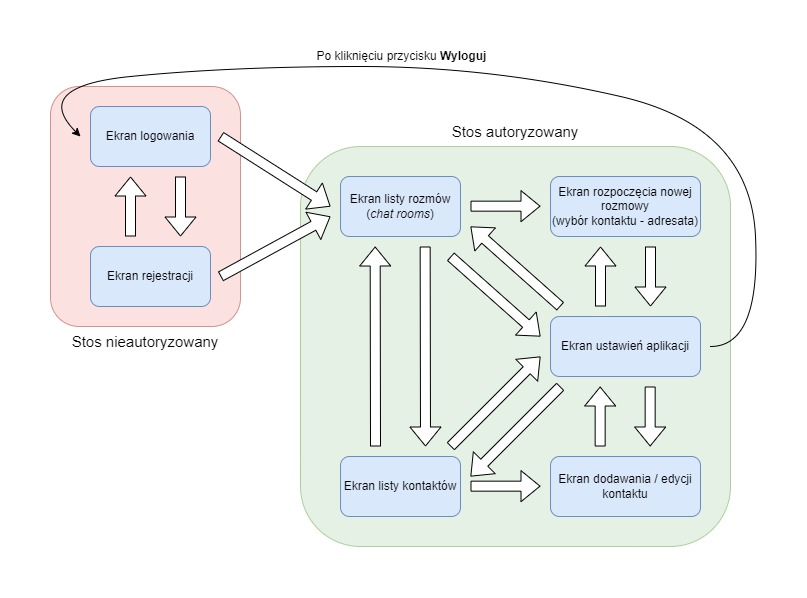
\includegraphics[scale=0.52]{views-map.jpg}
	\caption{Mapa widoków i możliwych przejść między nimi}
	\source{opracowanie własne}
	\label{fig:mobile_application_views_map}
\end{figure}

Wygląd poszczególnych widoków aplikacji przedstawiają zrzuty ekranów na Rysunkach \ref{fig:mobile_application_screenshots_1}-\ref{fig:mobile_application_screenshots_5}

\begin{figure}[H]
	\centering
	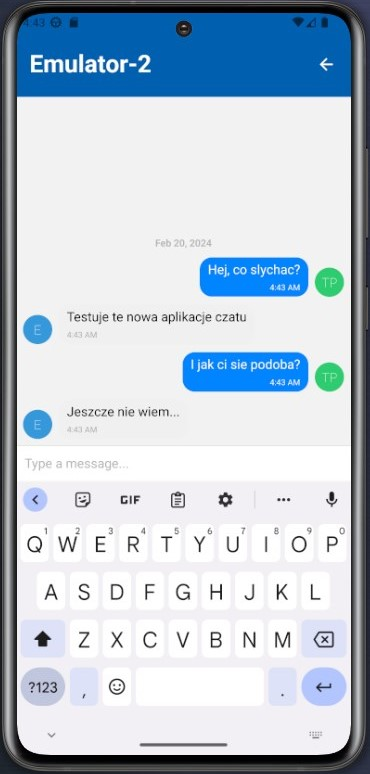
\includegraphics[scale=0.4]{ss_chat_screen.jpg}
	\caption{Ekran czatu}
	\source{opracowanie własne}
	\label{fig:mobile_application_screenshots_1}
\end{figure}

\begin{figure}[H]
	\centering
	\begin{tabular}{cc}
		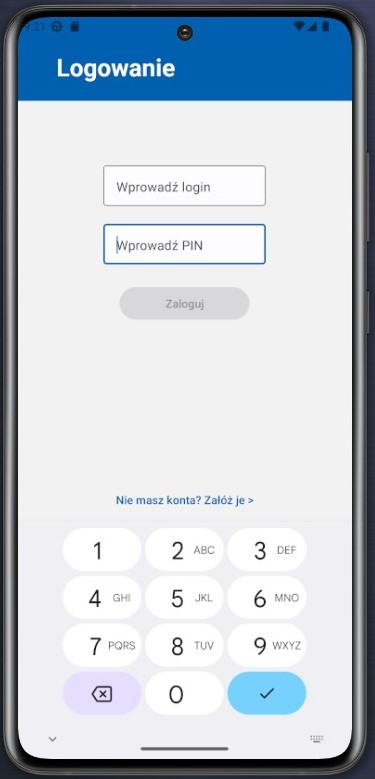
\includegraphics[scale=0.46]{ss_login_screen.jpg} & 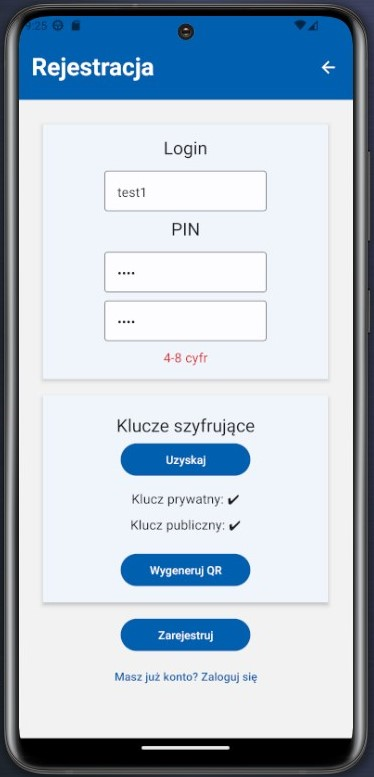
\includegraphics[scale=0.46]{ss_registration_screen.jpg} \\
		(a) Ekran logowania                               & (b) Ekran rejestracji                                    
	\end{tabular}
	\caption{Zrzuty ekranów aplikacji mobilnej}
	\source{opracowanie własne}
	\label{fig:mobile_application_screenshots_2}
\end{figure}

\begin{figure}[H]
	\centering
	\begin{tabular}{cc}
		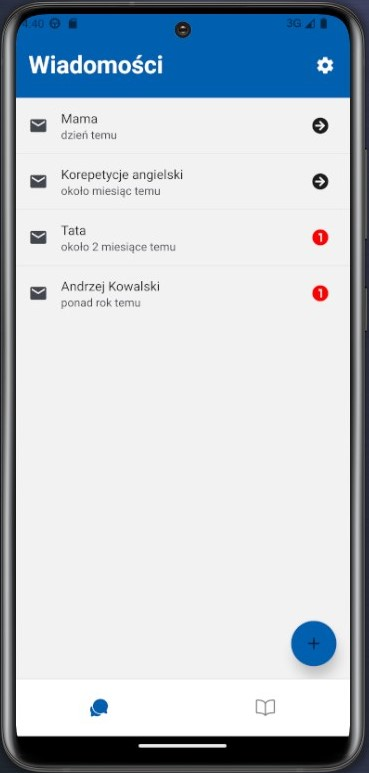
\includegraphics[scale=0.46]{ss_chat_rooms_screen.jpg} & 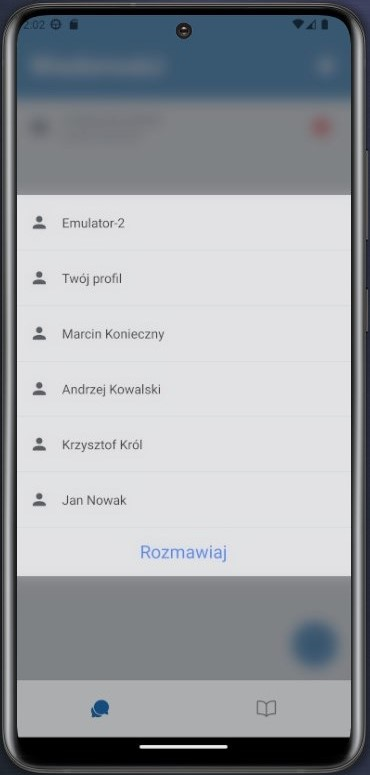
\includegraphics[scale=0.46]{ss_chat_room_create_screen.jpg} \\
		(a) Ekran listy rozmów                                & (b) Ekran tworzenia rozmowy                            
	\end{tabular}
	\caption{Zrzuty ekranów aplikacji mobilnej}
	\source{opracowanie własne}
	\label{fig:mobile_application_screenshots_3}
\end{figure}

\begin{figure}[H]
	\centering
	\begin{tabular}{cc}
		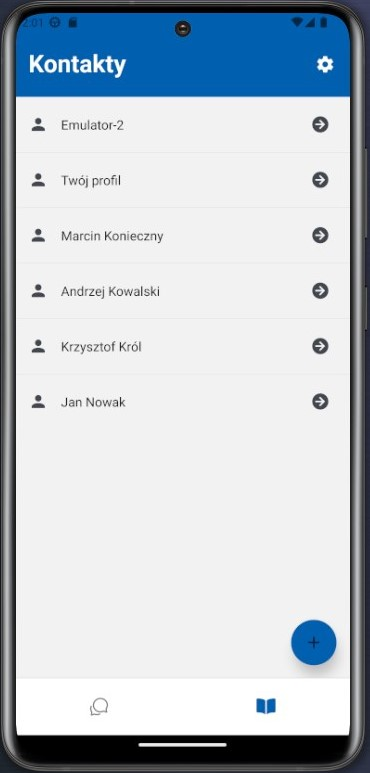
\includegraphics[scale=0.46]{ss_contacts_screen.jpg} & 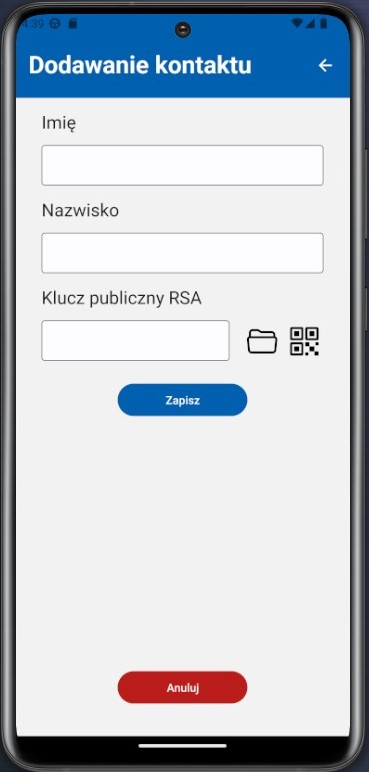
\includegraphics[scale=0.46]{ss_adding_contact_screen.jpg} \\
		(a) Ekran listy kontaktów                           & (b) Ekran tworzenia kontaktu                        
	\end{tabular}
	\caption{Zrzuty ekranów aplikacji mobilnej}
	\source{opracowanie własne}
	\label{fig:mobile_application_screenshots_4}
\end{figure}

\begin{figure}[H]
	\centering
	\begin{tabular}{cc}
		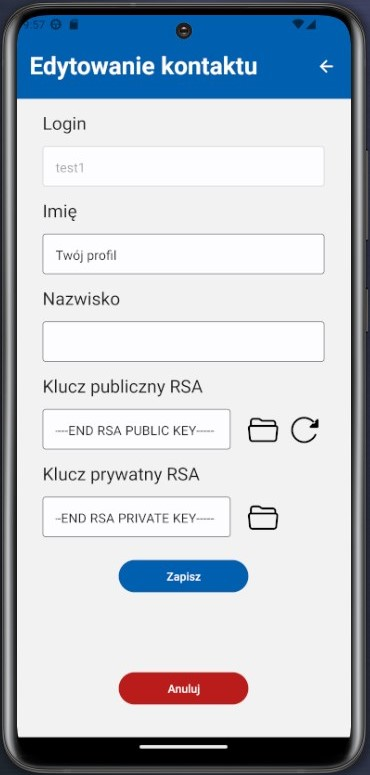
\includegraphics[scale=0.46]{ss_contact_edit_screen.jpg} & 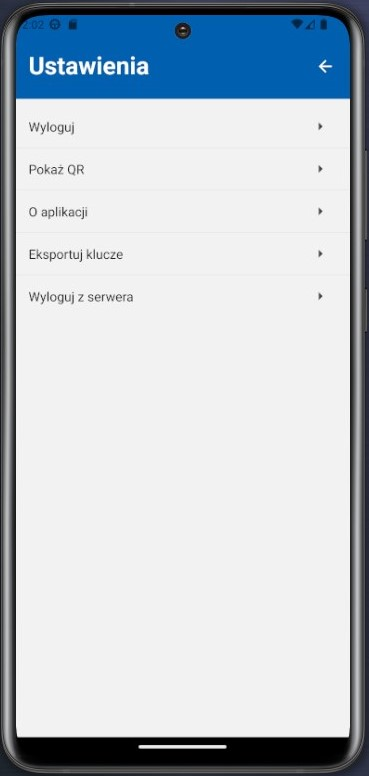
\includegraphics[scale=0.46]{ss_settings_screen.jpg} \\
		(a) Ekran edytowania kontaktu                  & (b) Ekran ustawień aplikacji                        
	\end{tabular}
	\caption{Zrzuty ekranów aplikacji mobilnej}
	\source{opracowanie własne}
	\label{fig:mobile_application_screenshots_5}
\end{figure}

\section{Realizacja funkcjonalności aplikacji}

Implementacja głównych funkcjonalności aplikacji wiąże się z szeregiem działań jakie musi wykonać klient mobilny oraz serwer. Poniżej przedstawione i opisane zostały główne funkcje aplikacji w formie diagramów procesów.

\begin{figure}[H]
	\centering
	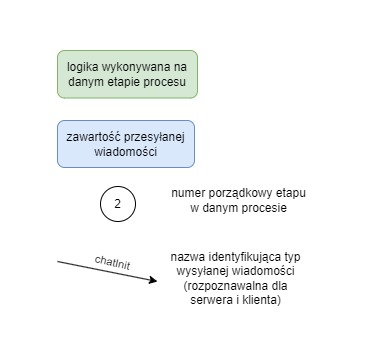
\includegraphics[scale=0.57]{oznaczenia-diagramow-procesow.jpg}
	\caption{Oznaczenia symboli na diagramach procesów}
	\source{opracowanie własne}
\end{figure}

\subsection{Nawiązywanie i zrywanie połączenia z serwerem}

Przy nawiązywaniu połączenia między aplikacją mobilną a serwerem generowany jest unikatowy identyfikator połączenia sesji (ang. \textit{session ID}, SID). Zadaniem serwera jest zapamiętanie powiązania klucz klienta - SID, jest to potrzebne przy realizacji innych procesów. Serwer aktualizuje dane w odpowiedzi na zmianę sytuacji (np. zerwanie połączenia i ponowne jego nawiązanie skutkuje uaktualnieniem powiązania klucz klienta - SID, a definitywne zerwanie połączenia - usunięciem tego wpisu z pamięci serwera).

\begin{figure}[H]
	\centering
	
\includegraphics[scale=0.41]{process-connect-diagram.jpg}
	\caption{Proces nawiązywania połączenia klienta z serwerem}
	\source{opracowanie własne}
\end{figure}

\begin{figure}[H]
	\centering
	
\includegraphics[scale=0.4]{process-disconnect-diagram.jpg}
	\caption{Proces zrywania połączenia klienta z serwerem}
	\source{opracowanie własne}
\end{figure}

\subsection{Uwierzytelnianie i rejestracja użytkownika}

W procesie uwierzytelniania wykorzystywane jest podpisywanie i weryfikowanie podpisu wiadomości kluczami RSA. Serwer generuje losowy ciąg znaków i przekazuje go klientowi, który podpisuje tę wiadomość przy pomocy swojego klucza prywatnego oraz odsyła ją do serwera. Następnie serwer przy pomocy klucza publicznego klienta weryfikuje poprawność wiadomości. Gwarantuje to, że użytkownik posiadający dany klucz publiczny posiada też odpowiadający mu klucz prywatny.

Ponadto serwer pobiera z bazy danych login i klucz publiczny, którymi identyfikuje się klient. W przypadku gdy w bazie danych nie ma tych wpisów, ale weryfikacja podpisu przebiegła pomyślnie następuje rejestracja użytkownika w bazie danych, po tym każda ponowna próba rejestracji na serwerze z tym loginem, ale innym kluczem publicznym lub z tym samym kluczem, ale innym loginem będzie odrzucana.

Użytkownik ma możliwość późniejszej zmiany klucza publicznego, ale jedynie w sytuacji gdy uzyskał autoryzację na serwerze w ramach danego połączenia.

\begin{figure}[H]
	\centering
	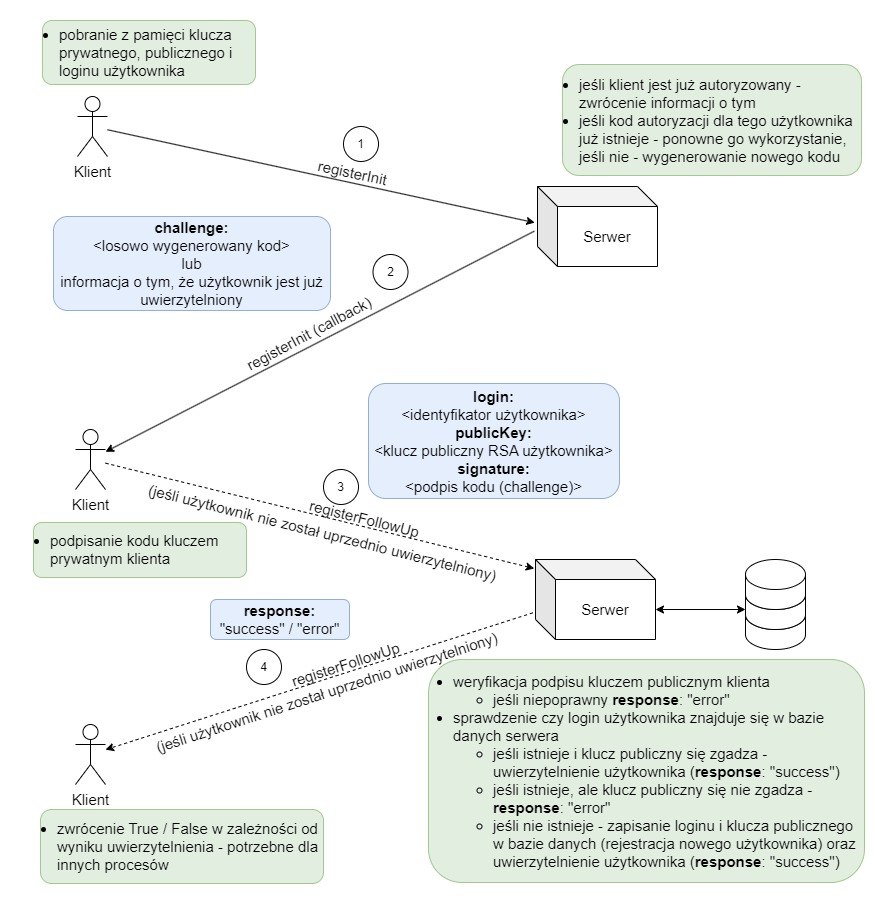
\includegraphics[scale=0.53]{process-authentication.jpg}
	\caption{Proces uwierzytelniania klienta na serwerze}
	\source{opracowanie własne}
\end{figure}

\subsection{Nawiązywanie komunikacji między użytkownikami}\label{sec:process-chat-initialization}

Wykorzystanie algorytmu SDEx do szyfrowania wiadomości między użytkownikami wymaga wymiany między nimi części klucza sesji $S1$ i $S2$. serwer pełni tu jedynie rolę pośrednika w wymianie wiadomości, ale sam nie ma wglądu w części klucza (są one przekazywane w postaci zaszyfrowanej przy pomocy kluczy RSA użytkowników) ani nie uczestniczy w szyfrowaniu i deszyfrowaniu wiadomości między użytkownikami, jest to wykonywane przez ich aplikacje klienckie.

\begin{landscape}
	\begin{figure}[H]
		\centering
		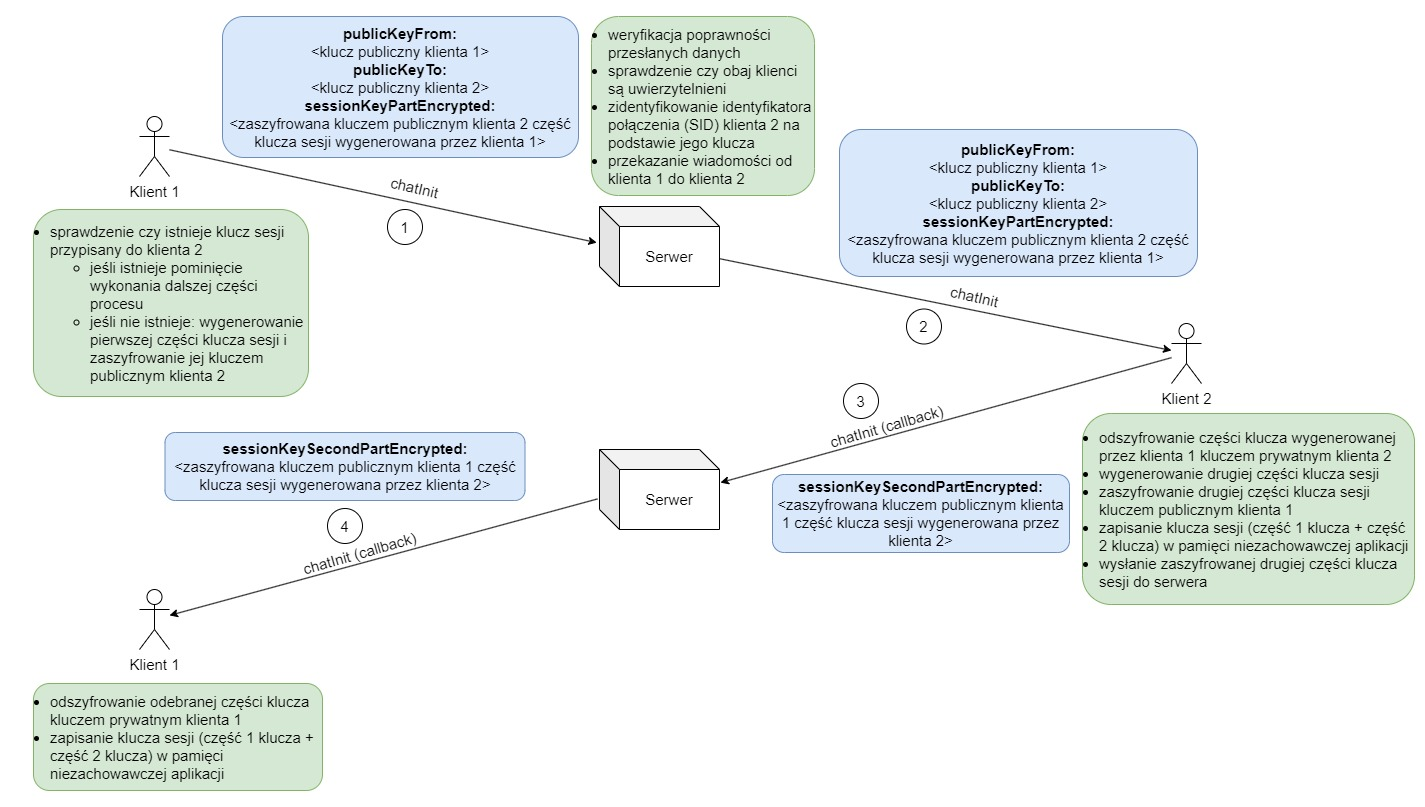
\includegraphics[scale=0.5]{process-chat-initialization.jpg}
		\caption{Proces nawiązywania komunikacji między użytkownikami}
		\source{opracowanie własne}
	\end{figure}
\end{landscape}

\subsection{Przekazanie wiadomości między użytkownikami}\label{sec:process-message-exchange}

Po uprzedniej inicjalizacji połączenia między klientami (Rozdział \ref{sec:process-chat-initialization}) użytkownicy posiadają uwspólniony klucz sesji, dzięki któremu są w stanie szyfrować i deszyfrować algorytmem SDEx wysyłane między sobą wiadomości.

Proces szyfrowania / deszyfrowania oraz przygotowania wiadomości do wysyłki (która oprócz treści zawiera metadane takiej jak klucz publiczny odbiorcy i adresata oraz datę utworzenia) przebiega w aplikacji mobilnej, natomiast serwer pośredniczy w przekazaniu tak przygotowanej wiadomości między użytkownikami (gdyż nie mają oni bezpośredniego połączenia między sobą). Serwer odpowiada także za zapewnienie autoryzacji obu klientów do wysyłki i odbioru wiadomości, sprawdza ich status dostępności, a na końcu zwraca potwierdzenie doręczenia i poprawnego odszyfrowania wiadomości przez odbiorcę do jej nadawcy. Na etapach oznaczonych na Rysunku \ref{fig:process-sending-message} numerami 2a i 3 jeśli nastąpi zerwanie połączenie Klienta 2 (odbiorcy wiadomości) z serwerem wiadomość zostaje uznana za niedostarczoną i serwer informuje o tym Klienta 1 (nadawcę) odpowiednio w kroku 2b lub 4. Komunikacja serwera z klientami toleruje opóźnienia w uzyskaniu odpowiedzi od odbiorców (tzw. \textit{timeout}) do 60 sekund. Po tym czasie serwer przestaje nasłuchiwać odpowiedzi i zwraca błąd doręczenia do nadawcy. Nie następuje ponowna próba doręczenia wiadomości przy wystąpieniu timeoutu lub utraty połączenia przez odbiorcę.

\begin{landscape}
	\begin{figure}[H]
		\centering
		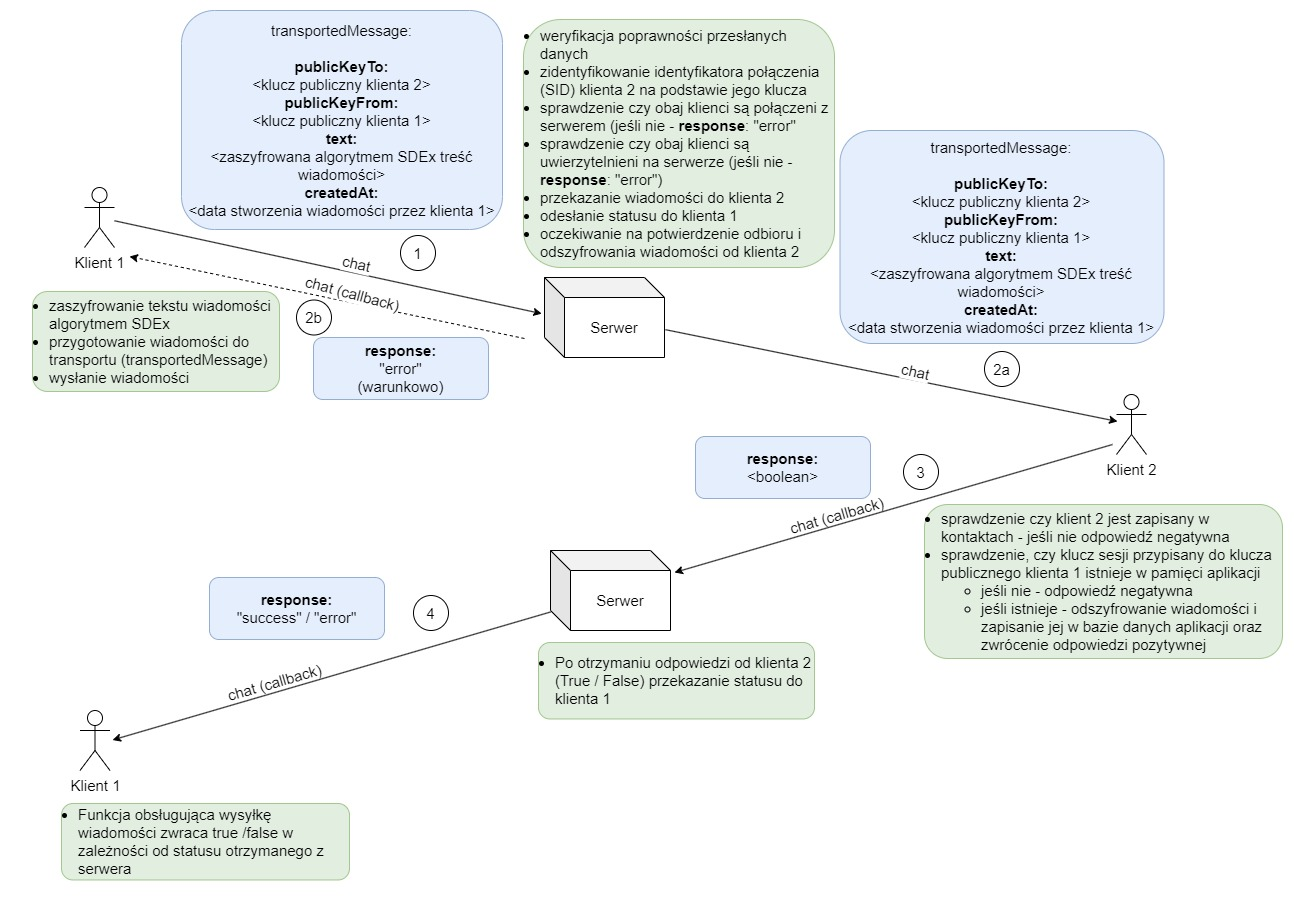
\includegraphics[scale=0.44]{process-sending-message.jpg}
		\caption{Proces przekazania wiadomości między dwoma użytkownikami}
		\source{opracowanie własne}
        \label{fig:process-sending-message}
	\end{figure}
\end{landscape}

\subsection{Sprawdzanie statusu połączenia innego klienta z serwerem oraz poprawności jego klucza publicznego}

Te dwie funkcjonalności mają charakter wspomagający dla procesów opisanych w rozdziałach \ref{sec:process-chat-initialization} i \ref{sec:process-message-exchange}. Dzięki ich zastosowaniu aplikacja może informować użytkownika próbującego przekazać wiadomość do jednego ze swoich kontaktów jeśli taka wymiana się nie powiedzie ze względu na to, że odbiorca nie jest połączony z serwerem lub że jego klucz publiczny nie został na nim zarejestrowany. Dzieje się to poprzez wyświetlenie baneru z odpowiednią wiadomością na ekranie czatu w aplikacji mobilnej (Rysunek \ref{fig:wrong-user-public-key-banner}).

\begin{figure}[H]
	\centering
	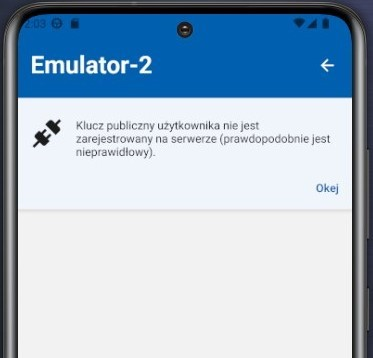
\includegraphics[scale=0.3]{ss_wrong-pub-key-banner.jpg}
	\caption{Baner informujący o niepoprawnym kluczu publicznym kontaktu}
	\source{opracowanie własne}
	\label{fig:wrong-user-public-key-banner}
\end{figure}

\begin{figure}[H]
	\centering
	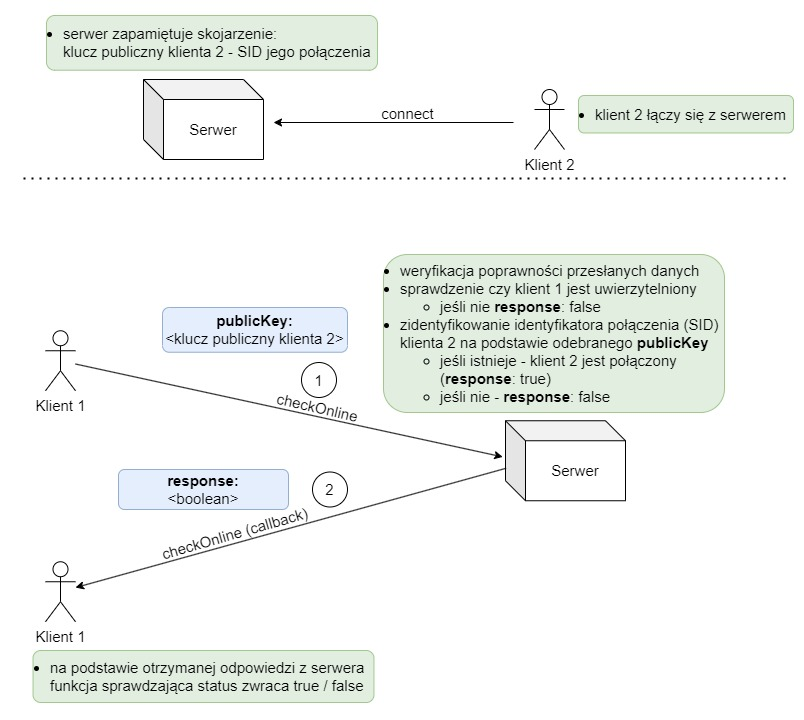
\includegraphics[scale=0.5]{process-check-user-online-status.jpg}
	\caption{Proces sprawdzania dostępności klienta na serwerze}
	\source{opracowanie własne}
\end{figure}

\begin{figure}[H]
	\centering
	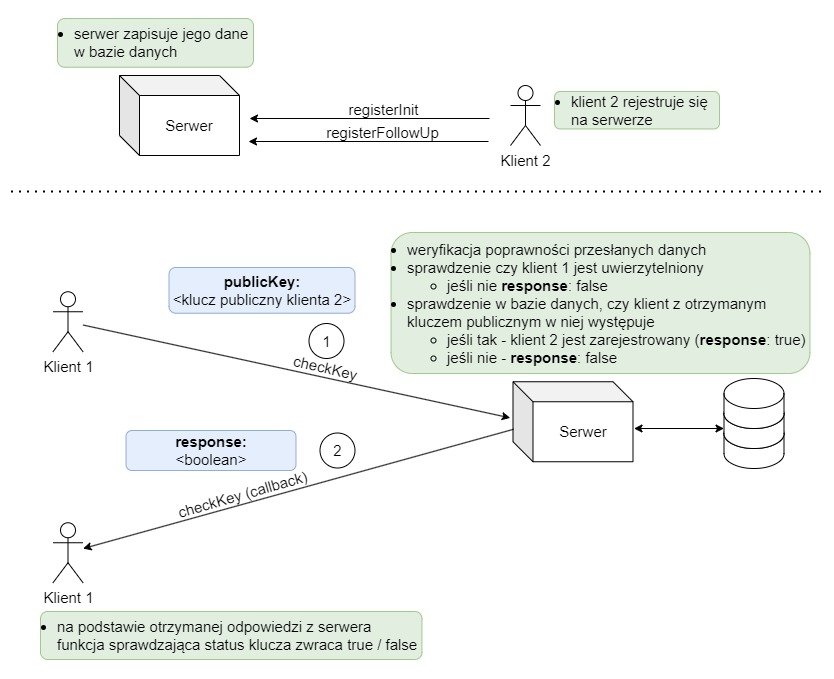
\includegraphics[scale=0.5]{process-check-user-public-key.jpg}
	\caption{Proces sprawdzania poprawności klucza publicznego klienta na serwerze}
	\source{opracowanie własne}
\end{figure}

\subsection{Zmiana klucza publicznego klienta na serwerze}

Zarejestrowany na serwerze użytkownik ma możliwość zmiany swojej pary kluczy RSA. Wykonywane jest to w aplikacji za pomocą formularza przedstawionego na Rysunku \ref{fig:mobile_application_screenshots_5} (a).

W wyniku tego konieczna jest zmiana klucza publicznego także na serwerze. Proces ten przedstawia Rysunek \ref{fig:user-public-key-change-process-diagram}. Co istotne, w przypadku niepowodzenia zmiany klucza publicznego na serwerze również w aplikacji mobilnej zmiana ta nie zostaje zapisana w pamięci zachowawczej aplikacji, w innym wypadku użytkownik trwale utraciłby możliwość uwierzytelnienia się na serwerze.

\begin{figure}[H]
	\centering
	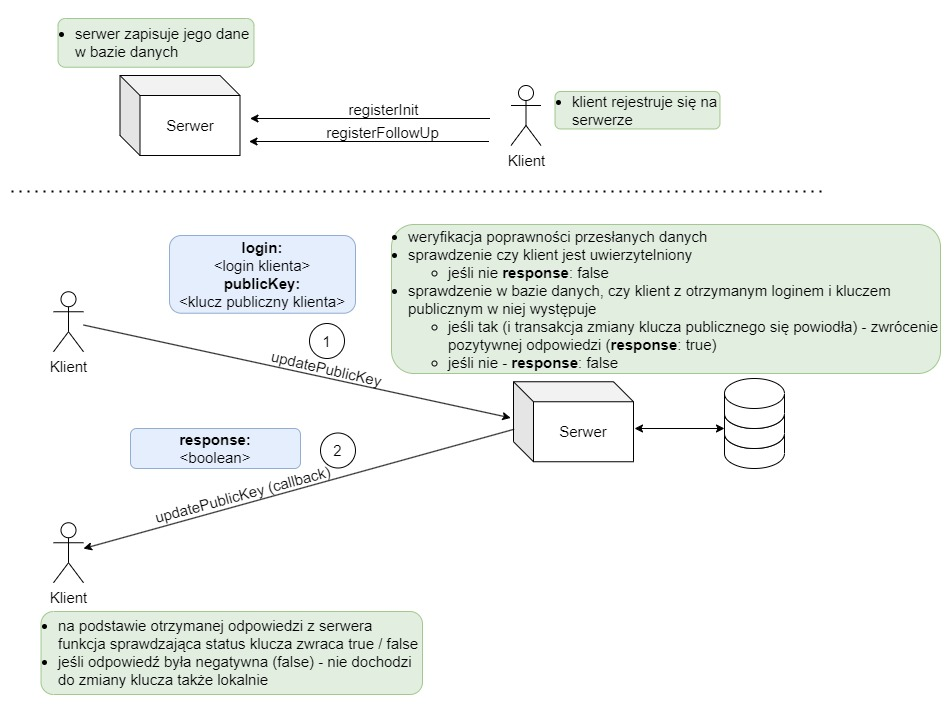
\includegraphics[scale=0.45]{process-change-user-public-key-on-server.jpg}
	\caption{Proces sprawdzania poprawności klucza publicznego klienta na serwerze}
	\source{opracowanie własne}
	\label{fig:user-public-key-change-process-diagram}
\end{figure}

\section{Wybrane fragmenty kodu aplikacji wraz z omówieniem}

Poniżej przedstawione są listingi kodu aplikacji, które wraz z komentarzem mają obrazować sposób implementacji rozwiązania. Są to fragmenty typowe (takie, które w podobnej formie pojawiają się w wielu miejscach w aplikacji) lub kluczowe z perspektywy problematyki podjętego opracowania - szyfrowania metodą SDEx. Z przytaczanych przykładów usunięto komentarze znajdujące się w kodzie oraz wywołania funkcji logujących informacje celem skrócenia listingów. Całość kodu aplikacji dostępna jest w załączonym do opracowania archiwum.

\subsection{Aplikacja mobilna}

Wysyłanie wiadomości zostało rozbite na kilka funkcji ze względu na złożoność tego procesu, oraz aby zachować odrębność odpowiedzialności między jednostkami kodu. Funkcja nadrzędna (Listing \ref{lst:js_send_message_main_function}) deleguje przygotowanie wiadomości w formacie przewidzianym do wysyłki (zaszyfrowane algorytmem SDEx oraz uzupełnione o metadane) do funkcji \code{prepareToSend} (Listing \ref{lst:js_prepare_to_send_message_function}). Sama natomiast odpowiada za pobranie wymaganych informacji (klucz nadawcy) z pamięci aplikacji oraz zarządzanie przebiegiem procesu w zależności od powodzenia lub niepowodzenia kolejnych jego etapów.

Samo wysyłanie wiadomości jest delegowane do funkcji \code{executeSendMessage} (Listing \ref{lst:js_execute_send_message_function}), która warunkując to powodzeniem dostarczenia wiadomości dodaje przesłaną wiadomość do lokalnej bazy danych, aby była widoczna w historii konwersacji. Jeśli natomiast wysyłka się nie powiedzie wiadomość nie jest zapisywana, dzięki temu obaj rozmówcy mają spójną historię rozmowy.

\begin{lstlisting}[caption={Wysyłanie wiadomości - funkcja nadrzędna},label={lst:js_send_message_main_function}]
export async function sendMessage(
    message: Message,
    publicKeyTo: string,
    sqlDbSession: WebSQLDatabase,
    sdexEngine: SdexCrypto,
): Promise<boolean> {
    const publicKeyFrom = mmkvStorage.getString("publicKey");
    if (!publicKeyFrom) {
        throw new PreconditionError(
            "[sendMessage] First party's key(s) not found. Cannot send message.",
        );
    }
    const transportReadyMessage: TransportedMessage = await prepareToSend(
        message,
        publicKeyFrom,
        publicKeyTo,
        sdexEngine,
    );
    message=${JSON.stringify(transportReadyMessage)}`);
    const successfulSend = await executeSendMessage(transportReadyMessage, message, sqlDbSession);
    if (successfulSend) {
        return true;
    }
    return false;
}
\end{lstlisting}

\begin{lstlisting}[caption={Przygotowywanie wiadomości do wysyłki},label={lst:js_prepare_to_send_message_function}]
export function prepareToSend(
    message: Message,
    publicKeyFrom: string,
    publicKeyTo: string,
    sdexEngine: SdexCrypto,
): TransportedMessage {
    const sdexEncryptedText = bytesToBase64(sdexEngine.encryptMessage(message.text));
    const sdexEncryptedImage = message.image
        ? bytesToBase64(sdexEngine.encryptMessage(message.image))
        : undefined;
    const sdexEncryptedVideo = message.video
        ? bytesToBase64(sdexEngine.encryptMessage(message.video))
        : undefined;
    const sdexEncryptedAudio = message.audio
        ? bytesToBase64(sdexEngine.encryptMessage(message.audio))
        : undefined;

    const sdexEncryptedMessage = new Message(
        message.contactIdFrom,
        message.contactIdTo,
        sdexEncryptedText,
        message.createdAt,
        message.unread,
        sdexEncryptedImage,
        sdexEncryptedVideo,
        sdexEncryptedAudio,
        message.id,
    );

    const transportedMessage = messageToTransportedMessage(
        sdexEncryptedMessage,
        publicKeyFrom,
        publicKeyTo,
    );

    return transportedMessage;
}
\end{lstlisting}

\begin{lstlisting}[caption={Wysyłanie wiadomości - funkcja odpowiedzialna za komunikację z serwerem i dodanie wiadomości do bazy danych},label={lst:js_execute_send_message_function}]
async function executeSendMessage(
    transportedMessage: TransportedMessage,
    message: Message,
    sqlDbSession: WebSQLDatabase,
): Promise<boolean> {
    try {
        const response = await socket.emitWithAck("chat", transportedMessage);
        if (response === "success") {
            try {
                await addMessage(message, sqlDbSession);
                return true;
            } catch (error) {
                return false;
            }
        } else {
            return false;
        }
    } catch (error) {
        return false;
    }
}
\end{lstlisting}

Kolejnym znaczącym przykładem jest proces wymiany kluczy sesji między użytkownikami oraz odpowiednie przechowanie go w pamięci niezachowawczej aplikacji. Klient wychodzący z inicjatywą komunikacji (co jest wywołane poprzez otwarcie okna czatu z wybranym przez siebie kontaktem) wywołuje funkcję \code{initiateChat} (Listing \ref{lst:js_initiate_chat_function}). Uzyskany klucz sesji jest przechowywany w pamięci. Implementacja sposobu przechowywania tej informacji w tzw. stanie aplikacji z użyciem biblioteki Zustand jest pokazana na Listingu \ref{lst:js_crypto_context}.

\newpage

\begin{lstlisting}[caption={Inicjowanie komunikacji z innym użytkownikiem},label={lst:js_initiate_chat_function}]
export async function initiateChat(publicKeyTo: string): Promise<boolean> {
    const existingSessionKey = useCryptoContextStore.getState().sdexEngines.has(publicKeyTo);
    if (existingSessionKey) {
        return true;
    }
    const firstPartyPublicKey = mmkvStorage.getString("publicKey");
    const firstPartyPrivateKey = mmkvStorage.getString("privateKey");

    if (!firstPartyPublicKey || !firstPartyPrivateKey) {
        throw new PreconditionError("First party's key(s) not found. Cannot initiate chat.");
    }

    const sessionKeyFirstPart = generateSessionKeyPart();
    const sessionKeyFirstPartString = bytesToBase64(sessionKeyFirstPart);

    const sessionKeyFirstPartEncrypted = await encryptRsa(publicKeyTo, sessionKeyFirstPartString);

    try {
        const response = await socket.emitWithAck("chatInit", {
            publicKeyFrom: firstPartyPublicKey,
            publicKeyTo,
            sessionKeyPartEncrypted: sessionKeyFirstPartEncrypted,
        });
        if (!response) {
            return false;
        }
        try {
            const sessionKeySecondPartString = await decryptRsa(firstPartyPrivateKey, response);
            const sessionKeySecondPart = base64ToBytes(sessionKeySecondPartString);
            const sessionKey = mergeUint8Arrays(sessionKeyFirstPart, sessionKeySecondPart);

            const sdexEngine = new SdexCrypto(sessionKey);
            useCryptoContextStore.getState().addUserEngine(publicKeyTo, sdexEngine);

            return true;
        } catch (error) {
            return false;
        }
    } catch (error) {
        return false;
    }
}
\end{lstlisting}

\vfill

\begin{lstlisting}[caption={Definicja jednego ze stanów aplikacji przechowującego informacje o kluczach sesji i odpowiadających im kontaktach},label={lst:js_crypto_context}]
export const useCryptoContextStore = create<CryptoContextState>((set) => ({
    sdexEngines: new Map<string, SdexCrypto>(),
    addUserEngine: (publicKey: string, sdexEngine: SdexCrypto): void => {
        set((prev) => ({
            sdexEngines: new Map(prev.sdexEngines).set(publicKey, sdexEngine),
        }));
    },
}));
\end{lstlisting}

Proces szyfrowania i deszyfrowania metodą SDEx opisany w sekcji \ref{sec:sdex_encryption_decryption} został zaimplementowany w sposób pokazany na Listingu \ref{lst:js_sdex_engine}

\begin{lstlisting}[caption={Szyfrowanie i deszyfrowanie metodą SDEx - implementacja},label={lst:js_sdex_engine}]
export default class SdexCrypto {
    HASH_LENGTH: number;
    ZEROED_BLOCK: Uint8Array;
    sessionKeyHash: Uint8Array;
    sessionKeyFirstPartHash: Uint8Array; // aka S1
    sessionKeySecondPartHash: Uint8Array; // aka S2

    constructor(sessionKey: Uint8Array, hashLength = 32) {
        this.HASH_LENGTH = hashLength;
        this.ZEROED_BLOCK = new Uint8Array(this.HASH_LENGTH);
        this.sessionKeyHash = this.blake3Wrapper(sessionKey);
        const [sessionKeyFirstPart, sessionKeySecondPart] = splitSessionKey(sessionKey);
        this.sessionKeyFirstPartHash = this.blake3Wrapper(sessionKeyFirstPart as Uint8Array);
        this.sessionKeySecondPartHash = this.blake3Wrapper(sessionKeySecondPart as Uint8Array);
    }

    blake3Wrapper(message: Uint8Array | string, context?: Uint8Array | string) {
        return blake3(message, {
            dkLen: this.HASH_LENGTH,
            context,
        });
    }

    static calculateBlock(block: Uint8Array, hash1: Uint8Array, hash2: Uint8Array): Uint8Array {
        if (block.length !== hash1.length || block.length !== hash2.length) {
            throw new SdexEncryptionError("[SdexCrypto.calculateBlock] Invalid block length");
        }
        return xorUintArrays(block, hash1, hash2);
    }

    calculateMessage(messageByteArray: Uint8Array): Uint8Array {
        const messageSplit = splitMessageIntoBlocks(messageByteArray, this.HASH_LENGTH);
        const messageBlocks = changeTo1IndexedArray(messageSplit);
        const result = <Uint8Array[]>[];
        const hashIterations = <Uint8Array[]>[]; // h0, h1, ..., hk

        result[1] = SdexCrypto.calculateBlock(
            messageBlocks[1] as Uint8Array,
            this.sessionKeyFirstPartHash,
            this.sessionKeyHash,
        );
        hashIterations[1] = this.blake3Wrapper(
            this.sessionKeyHash,
            mergeUint8Arrays(messageBlocks[1] as Uint8Array, messageBlocks[2] ?? this.ZEROED_BLOCK),
        );

        if (messageBlocks[2]) {
            result[2] = SdexCrypto.calculateBlock(
                messageBlocks[2],
                this.sessionKeyFirstPartHash,
                this.sessionKeySecondPartHash,
            );
            hashIterations[2] = this.blake3Wrapper(
                xorUintArrays(hashIterations[1], this.sessionKeyHash),
                mergeUint8Arrays(
                    messageBlocks[3] ?? this.ZEROED_BLOCK,
                    messageBlocks[4] ?? this.ZEROED_BLOCK,
                ),
            );
        }
        for (let k = 1; k <= messageBlocks.length; k += 1) {
            if (k >= 3) {
                hashIterations[k] = this.blake3Wrapper(
                    xorUintArrays(
                        hashIterations[k - 1] ?? this.ZEROED_BLOCK,
                        hashIterations[k - 2] ?? this.ZEROED_BLOCK,
                    ),
                    mergeUint8Arrays(
                        messageBlocks[2 * k - 1] ?? this.ZEROED_BLOCK,
                        messageBlocks[2 * k] ?? this.ZEROED_BLOCK,
                    ),
                );
                result[2 * k + 1] = SdexCrypto.calculateBlock(
                    messageBlocks[2 * k + 1] ?? this.ZEROED_BLOCK,
                    hashIterations[k] ?? this.ZEROED_BLOCK,
                    hashIterations[k - 1] ?? this.ZEROED_BLOCK,
                );
                result[2 * k + 2] = SdexCrypto.calculateBlock(
                    messageBlocks[2 * k] ?? this.ZEROED_BLOCK,
                    this.sessionKeySecondPartHash,
                    hashIterations[k] ?? this.ZEROED_BLOCK,
                );
            }
        }
        const nonEmptyArray = result.filter((element) => element);

        return mergeUint8Arrays(...nonEmptyArray);
    }

    encryptMessage(message: string): Uint8Array {
        const messageByteArray = stringToBytes(message);
        const encrypted = this.calculateMessage(messageByteArray);
        return encrypted;
    }

    decryptMessage(messageCipherTextByteArray: Uint8Array): string {
        const decryptedByteArray = this.calculateMessage(messageCipherTextByteArray);
        for (let i = decryptedByteArray.length - 1; i >= 0; i -= 1) {
            if (decryptedByteArray[i] !== 0) {
                const decrypted = bytesToString(decryptedByteArray.slice(0, i + 1));
                logger.debug(`[SdexCrypto.decryptMessage] (SDEx) Decrypted message: ${decrypted}`);
                return decrypted;
            }
        }
        return "";
    }
}
\end{lstlisting}

Najbardziej rozbudowanym pod względem funkcjonalności i zależności od różnych modułów aplikacji jest widok czatu, korzysta on zarówno w tle jak i w reakcji na działania użytkownika z szeregu funkcji komunikujących się z serwerem (np. aby sprawdzić status połączenia adresata i nadawcy z serwerem). Implementację tego widoku przedstawia Listing \ref{lst:js_chat_screen}.

Aby zapewnić odpowiednią responsywność aplikacji na przychodzące wiadomości (co jest szczególnie istotne gdy użytkownik jest w oknie czatu) podmieniono funkcję nasłuchującą wiadomości w tle na jej odpowiednik wywoływany bezpośrednio w komponencie definiującym widok czatu, dzięki temu w ramach tego widoku można natychmiast reagować na przychodzące tym kanałem wiadomości i odświeżać widok, aby wyświetlić otrzymaną wiadomość.

\begin{lstlisting}[caption={Implementacja ekranu czatu},label={lst:js_chat_screen}]
export default function Chat() {
    const [messages, setMessages] = React.useState<GiftedChatMessage[]>([]);
    const [contact, setContact] = React.useState<Contact | undefined>(undefined);
    const [firstPartyContact, setFirstPartyContact] = React.useState<Contact | undefined>(
        undefined,
    );
    const [bannerOfflineVisible, setBannerOfflineVisible] = React.useState<boolean>(false);
    const [thirdPartyOnline, setThirdPartyOnline] = React.useState<boolean>(true);
    const [thirdPartyKeyRegistered, setThirdPartyKeyRegistered] = React.useState<boolean>(true);
    const sqlDbSession = useSqlDbSessionStore((state) => state.sqlDbSession);
    const sdexEngines = useCryptoContextStore((state) => state.sdexEngines);
    const params = useLocalSearchParams();
    const contactId = params.contactId !== undefined ? Number(params.contactId) : undefined;

    React.useEffect(() => {
        requestRegister();
    }, []);
    
    React.useEffect(() => {
        socket.off("chat", outsideChatRoomChatListener);
        socket.on(
            "chat",
            async (
                message: TransportedMessage,
                callback: (response: boolean) => void,
            ): Promise<void> => {
                const sdexEngine = useCryptoContextStore
                    .getState()
                    .sdexEngines.get(message.publicKeyFrom);
                if (!sdexEngine) {
                    callback(false);
                    return;
                }
                const firstPartyPrivateKey = mmkvStorage.getString("privateKey");
                if (!firstPartyPrivateKey) {
                    callback(false);
                    return;
                }
                if (!sqlDbSession) {
                    callback(false);
                    return;
                }
                const contactFrom = await getContactByPublicKey(
                    message.publicKeyFrom,
                    sqlDbSession,
                );
                if (!contactFrom) {
                    callback(false);
                    return;
                }
                const decryptedMessage = await prepareToIngest(
                    message,
                    sdexEngine,
                    firstPartyPrivateKey,
                    contactFrom.id as number, // if it's fetched from db we know it has an id
                );
                await addMessage(decryptedMessage, sqlDbSession);

                if (firstPartyContact && contact?.id === decryptedMessage.contactIdFrom) {
                    const giftedChatMessage = messageToGiftedChatMessage(
                        decryptedMessage,
                        contact,
                        firstPartyContact,
                    );
                    setMessages([giftedChatMessage, ...messages]);
                }
                callback(true);
            },
        );
        return () => {
            socket.on("chat", outsideChatRoomChatListener);
        };
    }, []);

    React.useEffect(() => {
        if (contactId) {
            (async () => {
                const fetchedContact = await getContactById(Number(contactId), sqlDbSession);
                if (!fetchedContact) {
                    logger.error(
                        `[Chat.useEffect] User with contactId=${JSON.stringify(
                            contactId,
                        )} not found in storage.`,
                    );
                } else {
                    setContact(fetchedContact);
                }
                const fetchedFirstPartyContact = await getContactById(0, sqlDbSession);
                if (!fetchedFirstPartyContact) {
                    logger.error(
                        `[Chat.useEffect] First party contact info not found in the database..`,
                    );
                } else {
                    setFirstPartyContact(fetchedFirstPartyContact);
                }
            })();
        }
    }, [contactId]);

    function runOnlineCheck(publicKey: string) {
        checkOnline(publicKey)
            .then((online) => {
                logger.info(
                    `[Chat.useEffect] Third party connected is to the server: ${JSON.stringify(
                        online,
                    )}.`,
                );
                setThirdPartyOnline(online);
            })
            .catch((error: Error) => {
                logger.error(
                    `[Chat.useEffect] Error while checking if third party is online: ${error.message}`,
                );
            });
    }

    React.useEffect(() => {
        if (contact?.publicKey) {
            runOnlineCheck(contact.publicKey);
            const interval = setInterval(() => {
                runOnlineCheck(contact.publicKey);
            }, 10000);
            return () => clearInterval(interval);
        }
    }, [contact?.publicKey]);

    React.useEffect(() => {
        if (contact?.publicKey) {
            checkKey(contact.publicKey)
                .then((registered) => {
                    setThirdPartyKeyRegistered(registered);
                })
                .catch((error: Error) => {
                    logger.error(
                        `[Chat.useEffect] Error while checking if key is registered: ${error.message}`,
                    );
                });
        }
    }, [contact?.publicKey]);

    React.useEffect(() => {
        if (contact?.publicKey && sdexEngines.has(contact?.publicKey)) {
        } else if (
            socket.connected &&
            contact?.publicKey &&
            thirdPartyOnline &&
            !sdexEngines.has(contact.publicKey)
        ) {
            logger.info(`[Chat.useEffect] Sending "chatInit" message to ${contact.getFullName()}.`);
            void initiateChat(contact.publicKey);
        }
    }, [socket.connected, contact?.publicKey, thirdPartyOnline]);

    React.useEffect(() => {
        if (contact && contact.id && firstPartyContact) {
            (async () => {
                const messagesFromStorage = await getMessagesByContactId(
                    Number(contactId),
                    sqlDbSession,
                );
                await markMessagesAsRead(contact.id as number, sqlDbSession);
                const giftedChatMessages: GiftedChatMessage[] = [];
                messagesFromStorage.forEach((message) => {
                    giftedChatMessages.push(
                        messageToGiftedChatMessage(message, contact, firstPartyContact),
                    );
                });
                setMessages(giftedChatMessages);
            })();
        }
    }, [contact, firstPartyContact]);

    React.useEffect(() => {
        if (!socket.connected || !thirdPartyOnline || !thirdPartyKeyRegistered) {
            setBannerOfflineVisible(true);
        } else {
            setBannerOfflineVisible(false);
        }
    }, [thirdPartyOnline, socket.connected, thirdPartyKeyRegistered]);

    async function onSend(newMessages: GiftedChatMessage[] = []): Promise<void> {
        setMessages((previousMessages) => GiftedChat.append(previousMessages, newMessages));
        const thirdPartyCryptoEngine = sdexEngines.get(contact?.publicKey as string);
        if (
            contact &&
            socket.connected &&
            sqlDbSession &&
            thirdPartyCryptoEngine &&
            thirdPartyOnline
        ) {
            const results = [];
            for (const msg of newMessages) {
                const message = giftedChatMessageToMessage(msg, contact.id as number);
                results.push(
                    sendMessage(message, contact.publicKey, sqlDbSession, thirdPartyCryptoEngine),
                );
            }
            await Promise.all(results);
        }
    }

    function determineBannerText(): string {
        let text = "";
        if (!socket.connected) {
            text =
                "Brak połączenia z serwerem. Aby wysyłać i odbierać wiadomości, połącz się z serwerem.";
        } else if (!thirdPartyKeyRegistered) {
            text =
                "Klucz publiczny użytkownika nie jest zarejestrowany na serwerze (prawdopodobnie jest nieprawidłowy).";
        } else if (!thirdPartyOnline) {
            text =
                "Użytkownik jest offline. Możesz wysyłać wiadomości, ale nie ma gwarancji, że dotrą.";
        }
        return text;
    }

    function determineBannerActionLabel(): string {
        let text = "";
        if (!socket.connected) {
            text = "Polacz";
        } else if (!thirdPartyOnline || !thirdPartyKeyRegistered) {
            text = "Okej";
        }
        return text;
    }

    function determineBannerAction(): void {
        let action = () => {};
        if (!socket.connected) {
            action = socketConnect;
        } else if (!thirdPartyOnline) {
            action = () => setBannerOfflineVisible(false);
        }
        return action();
    }

    return (
        <SafeAreaView className="flex-1">
            <Appbar.Header style={styles.appBarHeader}>
                <Appbar.Content
                    title={contact ? contact.getFullName() : "<name>"}
                    titleStyle={styles.appBarTitle}
                />
                <Link href="/chats" asChild>
                    <Appbar.BackAction iconColor={styles.appBarIcons.color} />
                </Link>
            </Appbar.Header>
            <Banner
                visible={bannerOfflineVisible}
                icon="connection"
                actions={[
                    {
                        label: determineBannerActionLabel(),
                        onPress: determineBannerAction,
                    },
                ]}
            >
                {determineBannerText()}
            </Banner>
            <GiftedChat
                messages={messages}
                textInputProps={{ autoFocus: true }}
                onSend={(newMessages) => onSend(newMessages)}
                user={{
                    _id: 0,
                    name: firstPartyContact?.getFullName(),
                }}
            />
        </SafeAreaView>
    );
}
\end{lstlisting}

\subsection{Aplikacja serwerowa}

Większość funkcji obsługujących odbiór wiadomości od urządzenia klienckiego weryfikuje dane przychodzące. Zastosowano prostą logikę weryfikującą kompletność oraz typ wymaganych parametrów. Listing kodu \ref{lst:python_input_data_validation} pokazuje typową funkcję weryfikującą dane przychodzące dla wydarzenia finalizującego proces rejestracji na serwerze.

\begin{mypython}[caption={Walidacja danych przychodzących},label={lst:python_input_data_validation}]
def validate_register_follow_up_payload(data: Any) -> bool:
    if not isinstance(data, dict):
        return False
    if not data.get("login", None):
        return False
    if not data.get("publicKey", None):
        return False
    if not data.get("signature", None):
        return False
    return True
\end{mypython}

Endpoint obsługujący przekazywanie wiadomości między użytkownikami (Listing \ref{lst:python_transporting_message_mbetween_users}) jest przykładem ilustrującym implementację autoryzacji użytkownika do wykonywania pewnych akcji, a także pokazuje logikę obsługi trójstronnej komunikacji (klient 1 - serwer - klient 2).

\begin{mypython}[caption={Przekazywanie wiadomości między użytkownikami},label={lst:python_transporting_message_mbetween_users}]
@socket_manager.on("chat")  # type: ignore
async def handle_chat(sender_sid: str, data: Any) -> ResponseStatusType:
    if not validate_chat_payload(data):
        return "error"

    sender_key = PUBLIC_KEYS_SIDS_MAPPING.inverse.get(sender_sid, None)
    receiver_sid = PUBLIC_KEYS_SIDS_MAPPING.get(data["publicKeyTo"], None)
    if not sender_key or not receiver_sid:
        return "error"

    if not is_authenticated(sender_sid):
        return "error"
    if not is_authenticated(receiver_sid):
        return "error"

    try:
        receiver_response: bool = await socket_manager.call(
            "chat",
            data,
            to=receiver_sid,
        )
        if receiver_response:
            return "success"
        else:
            return "error"
    except TimeoutError:
        return "error"
\end{mypython}

\newpage

Operacje wykonywane na bazie danych (SQLite) pokazuje Listing \ref{lst:python_database_management}.

\begin{mypython}[caption={Implementacja menadżera bazy danych},label={lst:python_database_management}]
class DatabaseManager:
    def __init__(self, db_path: Path | str) -> None:
        try:
            self.client: sqlite3.Connection = sqlite3.connect(db_path)
        except Exception as e:
            raise DBConnectionError(e)

    def get_user_by_login(self, login: str) -> User | None:
        try:
            cursor: sqlite3.Cursor = self.client.execute(
                """
                SELECT
                    id, login, public_key
                FROM
                    users
                WHERE
                    login = :login;
                """,
                {"login": login},
            )
            output = cursor.fetchone()
            if not output:
                logger.info("User not found.")
                return None
            user = User(
                id=output[0],
                login=output[1],
                public_key=output[2],
            )
            logger.info("User data fetched successfully.")
            return user
        except Exception as e:
            raise DBConnectionError(e)

    def check_public_key(self, public_key: str) -> bool:
        try:
            cursor: sqlite3.Cursor = self.client.execute(
                """
                SELECT
                    *
                FROM
                    users
                WHERE
                    public_key = :key;
                """,
                {"key": public_key},
            )
            output = cursor.fetchone()
            log_msg = "Public key exists." if output else "Public key does not exist."
            logger.info(log_msg)
            return True if output else False
        except Exception as e:
            raise DBConnectionError(e)

    def update_user(self, login: str, new_public_key: str) -> bool:
        try:
            self.client.execute(
                """
                UPDATE
                    users
                SET
                    public_key = :new_public_key
                WHERE
                    login = :login;
                """,
                {
                    "new_public_key": new_public_key,
                    "login": login,
                },
            )
            self.client.commit()
            return self.client.total_changes > 0
        except Exception as e:
            raise DBConnectionError(e)

    def add_user(self, user: User) -> bool:
        try:
            self.client.execute(
                """
                INSERT INTO users (login, public_key)
                VALUES (:login, :public_rsa);
                """,
                {"login": user.login, "public_rsa": user.public_key},
            )
            self.client.commit()
            return self.client.total_changes > 0
        except Exception as e:
            raise DBConnectionError(e)

    def remove_user(self, login: str) -> bool:
        try:
            self.client.execute(
                """
                DELETE FROM
                    users
                WHERE
                    login = :login;
                """,
                {"login": login},
            )
            self.client.commit()
            return self.client.total_changes > 0
        except Exception as e:
            raise DBConnectionError(e)
\end{mypython}

\section{Testy}

Obie aplikacje zostały poddane testom mającym na celu usprawnienie pracy nad rozwijaniem omawianego oprogramowania oraz weryfikację poprawności stworzonego rozwiązania również w trakcie dalszej pracy nad kodem polegającej na jego optymalizacji i poprawy jakości (refactoringu).

Napisane zostały testy jednostkowe oraz integracyjne. Testowanie działania całości opisanych funkcjonalności (tzw. testy \textit{end to end}) oraz poprawności wyświetlania interfejsów graficznych przeprowadzono manualnie z użyciem emulatorów i fizycznych urządzeń z systemem Android.

Wybrane testy przedstawiają Listingi \ref{lst:sdex_test_suite}-\ref{lst:python_database_management_test}.


\begin{lstlisting}[caption={Testy jednostkowe sprawdzające implementację algorytmu SDEx},label={lst:sdex_test_suite}]
const sessionKey = new Uint8Array([
    199, 182, 158, 16, 28, 191, 237, 76, 143, 157, 160, 176, 212, 216, 69, 149, 116, 80, 98, 155,
    212, 183, 228, 53, 100, 16, 112, 89, 150, 82, 0, 116, 163, 242, 21, 164, 67, 83, 188, 5, 92, 26,
    189, 251, 17, 55, 89, 90, 4, 193, 80, 49, 150, 142, 205, 68, 98, 31, 22, 221, 192, 211, 235, 55,
]);
const clearTextMessage = "Hello world!";
const encryptedMessage = new Uint8Array([
    216, 52, 125, 5, 37, 138, 143, 114, 25, 15, 52, 201, 212, 18, 223, 193, 158, 24, 12, 232, 141,
    40, 144, 183, 142, 15, 134, 10, 228, 223, 72, 148,
]);
const sdexEngine = new SdexCrypto(sessionKey, 32);

test("Generating a session key part.", () => {
    const sessionKeyPart = generateSessionKeyPart(32);
    expect(sessionKeyPart.length).toBe(32);
});

test("Calculating a block properly.", () => {
    const array1 = new Uint8Array([121, 133]); //   01111001 10000101
    const array2 = new Uint8Array([38, 6]); //      00100110 00000110
    const array3 = new Uint8Array([130, 69]); //    10000010 01000101
    const result = SdexCrypto.calculateBlock(array1, array2, array3);
    const expected = new Uint8Array([221, 198]); // 11011101 11000110
    expect(result).toEqual(expected);
});

test("Calculating a block throws error on mismatching arrays lengths.", () => {
    const array1 = new Uint8Array([121, 133]);
    const array2 = new Uint8Array([9]);
    const array3 = new Uint8Array([130, 69]);
    const result = () => {
        SdexCrypto.calculateBlock(array1, array2, array3);
    };
    expect(result).toThrow(SdexEncryptionError);
    expect(result).toThrow("Invalid block length");
});

test("Encrypting a message properly.", () => {
    const result = sdexEngine.encryptMessage(clearTextMessage);
    expect(result).toEqual(encryptedMessage);
});

test("Decrypting a message properly.", () => {
    const result = sdexEngine.decryptMessage(encryptedMessage);
    expect(result).toBe(clearTextMessage);
});

test("SDEx encryption is reversible.", () => {
    const encrypted = sdexEngine.encryptMessage(clearTextMessage);
    const decrypted = sdexEngine.decryptMessage(encrypted);
    expect(clearTextMessage).toBe(decrypted);
});
\end{lstlisting}

\begin{lstlisting}[caption={Test integracyjny sprawdzający poprawność przygotowywania wiadomości do wysyłki, a następnie do jej zapisania u odbiorcy}]
test("Preparation process for message is fully reversible by ingestion process", async () => {
    const originalMessage = new Message(0, 1, "this is a test.", new Date("2023-01-02"), false);
    const senderPublicKey = `-----BEGIN PUBLIC KEY-----
  MIGfMA0GCSqGSIb3DQEBAQUAA4GNADCBiQKBgQCzc5oViIvknxXSbuIfqkyaZc1F
  nVvN52Buu136pSC6AbfVGX5KHzR7lzJl1ESxarREY8rrb8QxsNs+FAntuwiZopdW
  8f4zHB91neApkSLtuos4k6Gu78KvbldHkeCx8BdQsWz03lNXpv5REp9wNKGyzenw
  wF1dAlLOSg60efyUkwIDAQAB
  -----END PUBLIC KEY-----`;
    const receiverPublicKey = `-----BEGIN PUBLIC KEY-----
  MIGeMA0GCSqGSIb3DQEBAQUAA4GMADCBiAKBgFn8Dq9VxuIjiBzLmLZY5HUkHcr7
  czMdBKmsY3CiK6zauqmIXZqYLadVJBTh2+v2/kShiQViY+i9HbTJbzl7BTw6p8fr
  B0NWaNdlul/i0EkQZs45dJHe2HZebw7ZbOJmPyhUZAzmzastB7u69qNJANfxIFVB
  uII/u4ssaGki5iTJAgMBAAE=
  -----END PUBLIC KEY-----`;
    // for this test we skip combining session key parts and just provide a ready full length session key
    const senderSessionKey = generateSessionKeyPart(64);
    const sdexEngine = new SdexCrypto(senderSessionKey);

    const messageToSend = prepareToSend(
        originalMessage,
        senderPublicKey,
        receiverPublicKey,
        sdexEngine,
    );
    const ingestedMessage = prepareToIngest(messageToSend, sdexEngine, 1);
    expect(ingestedMessage.contactIdFrom).toEqual(1);
    expect(ingestedMessage.contactIdTo).toEqual(0);
    expect(ingestedMessage.text).toEqual(originalMessage.text);
    expect(ingestedMessage.createdAt).toEqual(originalMessage.createdAt);
    expect(ingestedMessage.image).toEqual(originalMessage.image);
    expect(ingestedMessage.video).toEqual(originalMessage.video);
    expect(ingestedMessage.audio).toEqual(originalMessage.audio);
});
\end{lstlisting}

\newpage

\begin{mypython}[caption={Testy jednostkowe sprawdzające operacje wykonywane na bazie danych},label={lst:python_database_management_test}]
import pathlib

import pytest

from sdex_server.database.database import DatabaseManager
from sdex_server.database.models import User


@pytest.fixture
def db_manager() -> DatabaseManager:
    db_path = pathlib.Path(__file__).parent.parent.parent / "resources" / "test-db.db"
    db_manager = DatabaseManager(db_path)
    return db_manager


@pytest.fixture
def user() -> User:
    return User(id=123, public_key="rsa-test", login="test_login")


@pytest.fixture
def updating_user(db_manager: DatabaseManager) -> bool:
    previous_user = User(public_key="old-rsa", login="some_user")
    new_user = User(public_key="new-rsa", login="some_user")
    yield db_manager.update_user(new_user.login, new_user.public_key)  # type: ignore
    db_manager.update_user(previous_user.login, previous_user.public_key)


@pytest.fixture
def adding_user(db_manager: DatabaseManager) -> bool:
    user_to_add = User(public_key="added-user-key", login="added-user")
    yield db_manager.add_user(user_to_add)  # type: ignore
    db_manager.remove_user(user_to_add.login)


@pytest.fixture
def deleting_user(db_manager: DatabaseManager) -> bool:
    user_to_delete = User(public_key="test-key", login="test123")
    yield db_manager.remove_user(user_to_delete.login)  # type: ignore
    db_manager.add_user(user_to_delete)


def test_get_user_by_login_returns_user(
    db_manager: DatabaseManager, user: User
) -> None:
    assert db_manager.get_user_by_login(user.login) == user


def test_get_user_by_login_doesnt_find_user(db_manager: DatabaseManager) -> None:
    assert db_manager.get_user_by_login("some_false_login") is None


def test_check_public_key_public_returns_public_key_exists(
    db_manager: DatabaseManager,
) -> None:
    assert db_manager.check_public_key("rsa-test") is True


def test_check_public_key_public_returns_public_key_doesnt_exist(
    db_manager: DatabaseManager,
) -> None:
    assert db_manager.check_public_key("false-rsa") is False


def test_update_user_executes_successfully(updating_user: bool) -> None:
    assert updating_user is True


def test_update_user_public_key_doesnt_find_user(
    db_manager: DatabaseManager, user: User
) -> None:
    assert db_manager.update_user("doesnt-exist", "some-key") is False


def test_add_user_inserts_user_successfully(adding_user: bool) -> None:
    assert adding_user is True


def test_remove_user_deletes_user_successfully(deleting_user: bool) -> None:
    assert deleting_user is True
\end{mypython}

\end{document}